\chapter{Коптилка}
%\corner{64}
\vepsianrose

Адмирал более\sdash менее выспался, но вылезать из палатки не спешил\mdash снаружи капал дождь. Замполит ещё спал, поэтому, чтобы не будить товарища, он достал судовой журнал и принялся записывать путевые заметки. Он каждый раз брал с собой этот журнал и каждый раз благополучно забывал его вести, но не в этом походе. Он~расписал по~свежим впечатлениям предыдущие два дня и~вспомнил, что обещал команде кофе к завтраку на днёвке.

\diagdash Шурик, там дождь чтоль?\mdash проснулся Замполит.

\diagdash Ну.

\diagdash Неохота вылазить$\ldots$

\diagdash А надо! Я вам кофеёк обещал. И у меня где\sdash то блинная мука была\mdash пойду оладьи соображу, а то каша чемпионов, поди, всем надоела уже.

\diagdash Фигасе разносолы. Я посплю ещё.

\newpage
\begin{wrapfigure}[13]{l}{0.5\textwidth}
	%\begin{figure}[h]
	\centering
	\includegraphics[width=0.47\textwidth]{47_1_coffee}
	\caption{\small\textit{...Кофеёк обещал...}}
	%\end{figure}
\end{wrapfigure}
Адмирал выполз из~палатки. Дождь почти закончился, но~погодка оставляла желать лучшего\mdash лес вокруг был влажным, дул неслабый ветерочек. Он~распалил костёр из~напиленных вчера впрок дров, поставил воду в~котелке на~чай\mdash всё равно кто\sdash нибудь да захочет чай\mdash и~принялся за кофе. Немного подумав, решил варить кофе на~газу, а~не~на~костре. Для этого он достал и~собрал свою мини\sdash горелку, собрал защитный экранчик от~ветра, поставил десантный котелок на синий цветок газа, щедро насыпал молотый кофе. Сверху он закрыл котелок подкотельником\mdash получилась как бы крышка\mdash так быстрее закипело. Народ потихоньку стал подтягиваться к~костру.

\diagdash Шу-у-урик, что варим?\mdash Серёга заспанно приземлился на брёвна.

\diagdash Кофе.

\diagdash Ва-а-ау.

\diagdash Ща, пару сек и будет готово!\mdash Адмирал дождался второго поднятия пенки и стал разливать всем желающим божественный напиток.\mdash Подставляйте!

Кофе вышел шикарным. Адмирал сдобрил его столовой ложкой белорусской сгущёнки и, развалившись в походном кресле, стал наслаждаться моментом.

\newpage

\begin{wrapfigure}[20]{r}{0.58\textwidth}
	%\begin{figure}[h]
	\centering
	\includegraphics[width=0.56\textwidth]{48_1_pancakes}
	\caption{\small\textit{...Принялся за оладьи...}}
	%\end{figure}
\end{wrapfigure}
\diagdash Шурик, такого ты ещё не делал.\mdash изрёк подошедший Замполит, тоже соблазнившись на~кофе.

\diagdash Не, помнишь, мы когда в последний раз по Чагодоще ходили, тоже кофеёк варили как\sdash то?

\diagdash А, тот наш <<арктический>> поход? Смутно~уже.

\diagdash Варили\sdash варили, было дело.\mdash подтвердил Серёга.

\diagdash Ну вот я решил повторить, так сказать.\mdash Адмирал вполне насладился напитком и принялся за оладьи. Он~достал из продуктовой гермы блинную муку и стал читать инструкцию на упаковке.

\diagdash Только не как в прошлый раз, ладно?\mdash посмеиваясь, напомнил Паша эпизод из их сплавного опыта, когда они на~днёвке близ Загривья на Чагодоще неудачно запекли целый котелок с~тестом.

\diagdash Там простая мука была, а то блинная. И сковородка у меня теперь нормальная, не очкуй.\mdash Адмирал согласно инструкции отмерил пропорции и принялся замешивать тесто в~круглом пашином подкотельнике, который как нельзя лучше подошёл для этой цели.

Оладьи стали выпекаться вполне себе приличными, Адмирал даже не ожидал. Спустя минут 15 на перевёрнутой крышке котелка образовалась целая горка аппетитно пахнущих оладушек. Паша достал невесть откуда взявшиеся остатки копчёного рулета и прочего по мелочи, народ засел за трапезу:

\diagdash Шурик, а неплохо!

\diagdash Ну!

\diagdash Лучше, чем тот запечённый котелок, аха-ха!\mdash припомнил Паша.

\diagdash Однозначно. Опыт растёт!

После все разбрелись кто куда\mdash Замполит с Серёгой взяли пилу и пошли делать <<кружочки>>\mdash спилы сосновых поленьев\mdash на память в качестве сувениров, Руслан в~походном кресле кайфовал у костра, Паша засобирался на~рыбалку в залив, а Адмирал, сварив себе ещё порцию кофе и~раскурив сигару, снова принялся за путевые заметки.

Серёга с Замполитом напилили <<кружочков>> и~притащили их к костру похвастаться:

\diagdash Мы такие, короче, в детстве с каждого сплава притаскивали, потом сушили дома, и типа память о~сплаве оставалась.\mdash поделился воспоминаниями Замполит.

\diagdash Сушить только в~пакете надо, а то треснет спил, наверно.\mdash предположил Серёга.

\diagdash Логично. Надо тоже себе напилить потом.\mdash согласился Адмирал,\mdash я думаю можно на них чё\sdash нить выжечь на память. Типа там <<Суна>> и год? М? Что скажете?

\diagdash И лаком вскрыть. А то они темнеют потом.\mdash посоветовал Замполит.

\diagdash Да, неплохая идея. Замётано. Так. Серёг, а ягоды вроде оставались же ещё?\mdash спросил Адмирал, повернувшись к тому.

\diagdash Да, вот в пятилитрашке. Компотика наварить?

\diagdash Было бы клёво.

\diagdash Щас сделаем.\mdash Серёга сходил зачерпнул котелок воды.

Спустя совсем немного времени компот был готов:

\diagdash Нава-а-аристо!

\diagdash А то!

\diagdash Серёга у нас главный по компотам в~этом сплаве.\mdash попробовал компот Руслан.

\begin{wrapfigure}[10]{r}{0.51\textwidth}
	%\begin{figure}[h]
	\centering
	\includegraphics[width=0.49\textwidth]{49_1_kompot}
	\caption{\small\textit{...Нава-а-аристо!..}}
	%\end{figure}
\end{wrapfigure}

\diagdash Не, по~компотикам главный\mdash Замполит, а~Серёга по~сборке голубики.\mdash не преминул подколоть Замполита Адмирал.

\diagdash Ой да харош, Шурик!\mdash Замполит как раз попробовал варево,\mdash М\sdash м\sdash м, зачёт!

\diagdash Ы-ы-ы!

\newpage
\diagdash Ладно, чем занимаемся сегодня?

\diagdash Чилим. Хочется насладиться природой, это же последняя стоянка\mdash потом завтра переход через озеро, и~мы~в~Гирвасе.\mdash Адмирал развалился в кресле с~сигарой.

\diagdash Лад\'{ы}. Тогда я\mdash на рыбалку.\mdash ответил Паша.

\diagdash Я\mdash за черникой.\mdash сказал Серёга. Руслан присоединился к нему, и они, взяв 5\sdash литровую бутыль с~обрезанным верхом, пошли ещё за ягодами для компота.

Паша отошёл от лагеря буквально метров на 50 и~расположился со стульчиком на берегу озера. Достал удочку, снасти, подобрал наживку, закинул и стал умиротворённо ждать, временами подкармливая рыбу остатками завтрака. %Спустя немного времени решил прикормить. %И тут попёрло! Он стал вытягивать буквально одну за одной!

Адмирал решил немного обследовать местность дальше вглубь мыса, на котором они устроили свою последнюю стоянку, днёвку. Он от души полил штаны и штормовку дэтой\footnote{ДЭТА (диэтилтолуамид)\mdash химическое соединение, широко применяемое в средствах для отпугивания кровососущих насекомых, в~т.ч.~клещей.} и~направился в~лес\mdash обогнул их лагерь, проведав как дела у~Паши и,~оставив в~стороне Серегу с Русланом, собиравших ягоды, стал подниматься по пологому склону, поросшему высокими красивыми соснами. 

Местность была завораживающе красива\mdash Адмирал, дойдя до вершины холма, обернулся. Его взгляду предстал вид на средней частоты светлый карельский сосновый лес, где внизу на самом мысу находилась их стоянка и~виднелся костёр, у~которого остался Замполит. Ветер, дувший с северо\sdash запада, с Суны, был достаточно тёплым по карельским меркам, и заставлял лесное великолепие пошумливать кронами. Высоченные сосны покачивались на~ветру, чуть поскрипывая. Адмирал замер в немом оцепенении, всеми фибрами души впитывая эту красоту. Ему так хотелось каким\sdash нибудь неведомым образом остановить время и продлить наслаждение этим моментом, этими видами, этими запахами соснового бора$\ldots$ 

Он шёл всё дальше вглубь мыса, пока наконец не зашёл в~абсолютные дебри. <<Класс,\mdash думалось ему,\mdash и почему нельзя тут жить?>> И тут же внутренний голос объяснял ему: <<А работать где будешь? А кушоц чего? Да и климат суров, забыл?>> Нехотя Адмирал признавал правоту внутреннего голоса, но от этого легче не становилось абсолютно. Вместо просто наслаждения созерцанием окружающей природы, Адмиралу было безумно горько от того, что завтра это всё закончится, и снова наступят серые будни, город, работа и~опять всё по\sdash новой, как будто и~не~было ни~порогов на~Нурмисе, ни~робинзоновой стоянки на~острове, как будто не~штурмовали два дня подряд пороги$\ldots$ 

<<Ау, очнись! Как не~было! Было ещё как! Осело в~мозгу так, что фиг выпрешь!>>\mdash тут~же напомнил внутренний голос. <<Брысь!>>\mdash Адмирал прогнал все мешающие мысли и~уселся на~поваленное дерево медитировать$\ldots$ Медитировать он, конечно, не~умел, но~поджал под себя ноги на манер позы лотоса, положил кисти рук, обращённые к~небу, на~колени, выпрямил спину и попытался максимально отключиться от бытия, воспарить над лесом, над рекой, над ощущением собственного <<я>> в~попытке ощутить себя не~просто неотъемлемой частью природы, а~самой природой.

<<Я обязательно вернусь сюда ещё раз\mdash этот маршрут стоит того, чтобы пройти его ещё разок\sdash другой>>,\mdash подумал Адмирал и, медленно очнувшись от~медитации спустя где\sdash то часа два, пошёл обратно в~лагерь.

%\diagdash Компот\'{и}н-антипохмел\'{и}н, ы-ы-ы!

\newpage

\begin{wrapfigure}[22]{l}{0.58\textwidth}
	%\begin{figure}[h]
	\centering
	\includegraphics[width=0.56\textwidth]{50_1_fishsmoke}
	\caption{\small\textit{...Переворачивал рыбу...}}
	%\end{figure}
\end{wrapfigure}
В лагере творился движ\mdash Паша наловил немерено рыбы и решил её закоптить. Для этой цели он соорудил донельзя простую коптилку\mdash вырыл сапёрной лопаткой небольшую яму, развёл там костерок и заложил сверху ольховыми ветками с сочной листвой. Зелёная сырая листва сбила пламя, и всё это начало неслабо дымить. Прямо сверху на~листья, через которые валил дым, он разложил свой улов, параллельно продолжая рыбачить, пополняя коптилку.

\diagdash Вот это нифига себе!\mdash воскликнул Адмирал, возвратившись из леса.

\diagdash А ты думал? Пока ты там прохлаждаешься непонятно где, тут вона чё!\mdash Пашка, щурясь от дыма, переворачивал рыбу.

\diagdash Офигенно!!!

\diagdash А парни лисичек настригли, вон, иди глянь.

Адмирал вернулся к костру, где Серёга с Русланом чистили грибы:

\diagdash Серёг, ты, наверно, в жизни столько грибов с ягодами не собирал, как в этом сплаве?

\diagdash Ну не то, чтобы прям совсем в жизни, но да, богато, очень богато собрали, погляди!\mdash Серёга протянул ему котелок, доверху забитый отборными лисичками.

\diagdash Супер! А ты знаешь, что они никогда не~бывают червивыми?

\diagdash Да ну?

\diagdash Ну да! Только если совсем большие экземпляры, да~и~то в~сухой~год.

\diagdash А почему?

\diagdash Там в них какая\sdash то химоза есть, её черви не любят.

\diagdash А на человека как эта химоза?

\diagdash Да никак, всю жись ели, ы\sdash ы\sdash ы!\mdash заржал Адмирал.\mdash Вкуснотища же! Вы тогда промойте и почистите их, а я лука начищу и зажарим енто всё дело к рыбе копчёной. Будет офигенский обед!

\diagdash Ага!

В это время с озера донёсся нарастающий шум моторки, все обернулись:

\diagdash По\sdash моему на нас чешет прям?

\diagdash Да не, щас свернёт, чё ему тут надо\sdash то?

\diagdash Да вот не сворачивает$\ldots$

Через пару минут мужик на надувной моторке подошёл к мысу. На лодке было не меньше пяти удочек в креплениях:

\diagdash Здарова! Л\'{о}вите?

\diagdash Ловим.\mdash нехотя ответил Адмирал.

\diagdash И как, есть чё?

\diagdash Не, нету нифига, вообще не клюёт.\mdash не поведя бровью, ответил Паша.

\diagdash Вот и у меня! Закурить\sdash то есть?\mdash не унимался мужик.

\diagdash Нету, дядь! Конец похода\mdash всё кончилось!\mdash мгновенно нашёлся Адмирал.

\diagdash Ну бывайте!\mdash мужик отошел подальше от берега на~реверсе и, развернувшись, пошёл на~полной скорости против течения Суны. 

\diagdash Умник, блин! Рыбу ему покажи, закурить дай! Такому палец дай, по локоть откусит. Ещё б налить попросил.\mdash возмутился Паша.

\diagdash Хрен ему.\mdash резюмировал Адмирал.\mdash Человеческий фактор, ничё не попишешь.

Рыба стала поспевать с копчения. Паша свернул удочку и отправился снимать готовую рыбу с коптилки:

\diagdash Подсобите, парни?

Серёга занимался лисичками у костра, а Адмирал\mdash луком. Руслан с Замполитом взяли крышки от котелков в~качестве тарелок и пошли за Пашей. Спустя пару минут они принесли к костру безумно вкусно пахнущую рыбу:

\diagdash Это фантастика!

\diagdash Кормилец наш, Паш!\mdash Адмирал отложил лук и принялся уплетать рыбу, разломив её пополам по~хребтине.\mdash М\sdash м\sdash м, вкуснотища!

\diagdash А то! Обращайтесь!\mdash Паша довольный тоже сидел у костра и наворачивал.

\diagdash Так, а у нас картошки остаётся сверх нормы, можно замутить грибы с картошкой.\mdash сообразил Адмирал.

\diagdash Погодь, дай рыбкой насладиться!\mdash доносились звуки поглощения копчёного лакомства.

\diagdash Я чёт не подумал, что коптилку так просто можно сделать\mdash из ямы, фактически.\mdash признался Адмирал, наворачивая за обе щеки очередную копчёную рыбку.

\diagdash Ну да\mdash яма, листья, что ещё надо то?

\diagdash Рыба, рыба нужна, ну? Без Паши б~не~было ничего. Замполит, впечатления?\mdash Адмирал повернулся к тому.

\diagdash Оч вкусно, Шурик. Прям от души, в охотку!

Копчёная рыба исчезла за 15 минут, не больше. Адмирал докончил с луком и картошкой, а Серёга дочистил и промыл грибы:

\diagdash Шу-у-урик, готово!

\begin{wrapfigure}[12]{l}{0.58\textwidth}
	%\begin{figure}[h]
	\centering
	\includegraphics[width=0.56\textwidth]{51_1_mushrooms}
	\caption{\small\textit{...Жарим!..}}
	%\end{figure}
\end{wrapfigure}\diagdash Ну, жарим!\mdash Адмирал присел к~костру со~своей алюминиевой сковородочкой, отвалил головешку на~манер плиты и~приступил к~жарке.\mdash Пошарь там в гермах, майонез должен был остаться ещё.\mdash Шурик щурился от дыма костра.

\begin{wrapfigure}[11]{l}{0.58\textwidth}
	%\begin{figure}[h]
	\centering
	\includegraphics[width=0.56\textwidth]{52_1_delight}
	\caption{\small\textit{...Адмирал закрыл глаза...}}
	%\end{figure}
\end{wrapfigure}
Блюдо вышло, как и вся еда на~костре, естественно, восхитительным\mdash когда всё было готово, команда вновь расселась в~кружок и навернула лисичек с~картошкой. Адмирал закрыл глаза от удовольствия:

\diagdash М-м-м! По красоте, парни?

\diagdash Спрашиваешь? Кулинар$\exldots$%!$\ldots$

$\ldots$День проходил у них в чревоугодии и лености, народ полностью расслабился и отдыхал. На мысу, если очень\sdash очень  постараться, ловила мобильная связь. Все уже набрали домой смс\sdash ки или позвонили родным. Адмирал, зачерпнув кружечку компотика из котелка, уселся в кресло, открыл свой командирский планшет и включил мобильник:

\diagdash Так, парни, получается, что сегодня воскресенье. Мы~прошли маршрут на 1 день быстрее плана.

\diagdash Как так?\mdash поинтересовался Серёга.

\diagdash Ну я изначально планировал с запасом на один экстренный день, если вдруг придётся ремонтировать байдарки после порогов. Перестраховался, так скажем.

\diagdash А-а-а.\mdash протянул Серёга.\mdash И чего теперь?

\diagdash Да ничего, надо Олегу отзвониться насчёт машин\mdash он просил с~Викшозера позвонить за сутки.

\diagdash Шурик, а мы не на Викшозере, а на Лавалампи!\mdash угорал Замполит, тоже открыв карту в мобильнике.

Тот закатил глаза:

\diagdash Ну это одно и то же, тут деление\sdash то весьма условное. Можно вообще сказать, что мы на~Суне ещё стоим, в~самом устье.\mdash и~набрал Олегу.

После Адмирал вспомнил про свою кружку с компотом, который давно остыл, и, снова открыв судовой журнал, принялся дописывать путевые заметки, раскурив сигару.

\diagdash Шурик, смотришься на все сто.\mdash Замполит с~Серёгой фотографировали всех и вся на память.

\diagdash Ну!\mdash тот закинул ногу на ногу и самозабвенно выводил строчку за строчкой простым карандашом.

\diagdash Шурик, почему простым карандашом?

\diagdash Моряцкая мудрость! Он не смывается водой, прикинь? Это мне один капитан 1 ранга поведал.

\diagdash Ты собрался топить судовой журнал?\mdash Паша сидел и~мешал сахар в~чае сосновой веточкой.

\diagdash Так\sdash то нет, но завтра у нас переход по~огроменному озеру$\ldots$

\diagdash Ой~да~харош! Не~стращай народ.

\diagdash И~в~мыслях нет. Просто на большой воде всё~же не~так комфортно себя ощущаешь в~байдарке.

\diagdash Да я б не сказал. А в порогах, что, комфортно?

\diagdash Да тож не очень, особенно когда заливает сверху волной.

\begin{wrapfigure}[17]{l}{0.50\textwidth}
	%\begin{figure}[h]
	\centering
	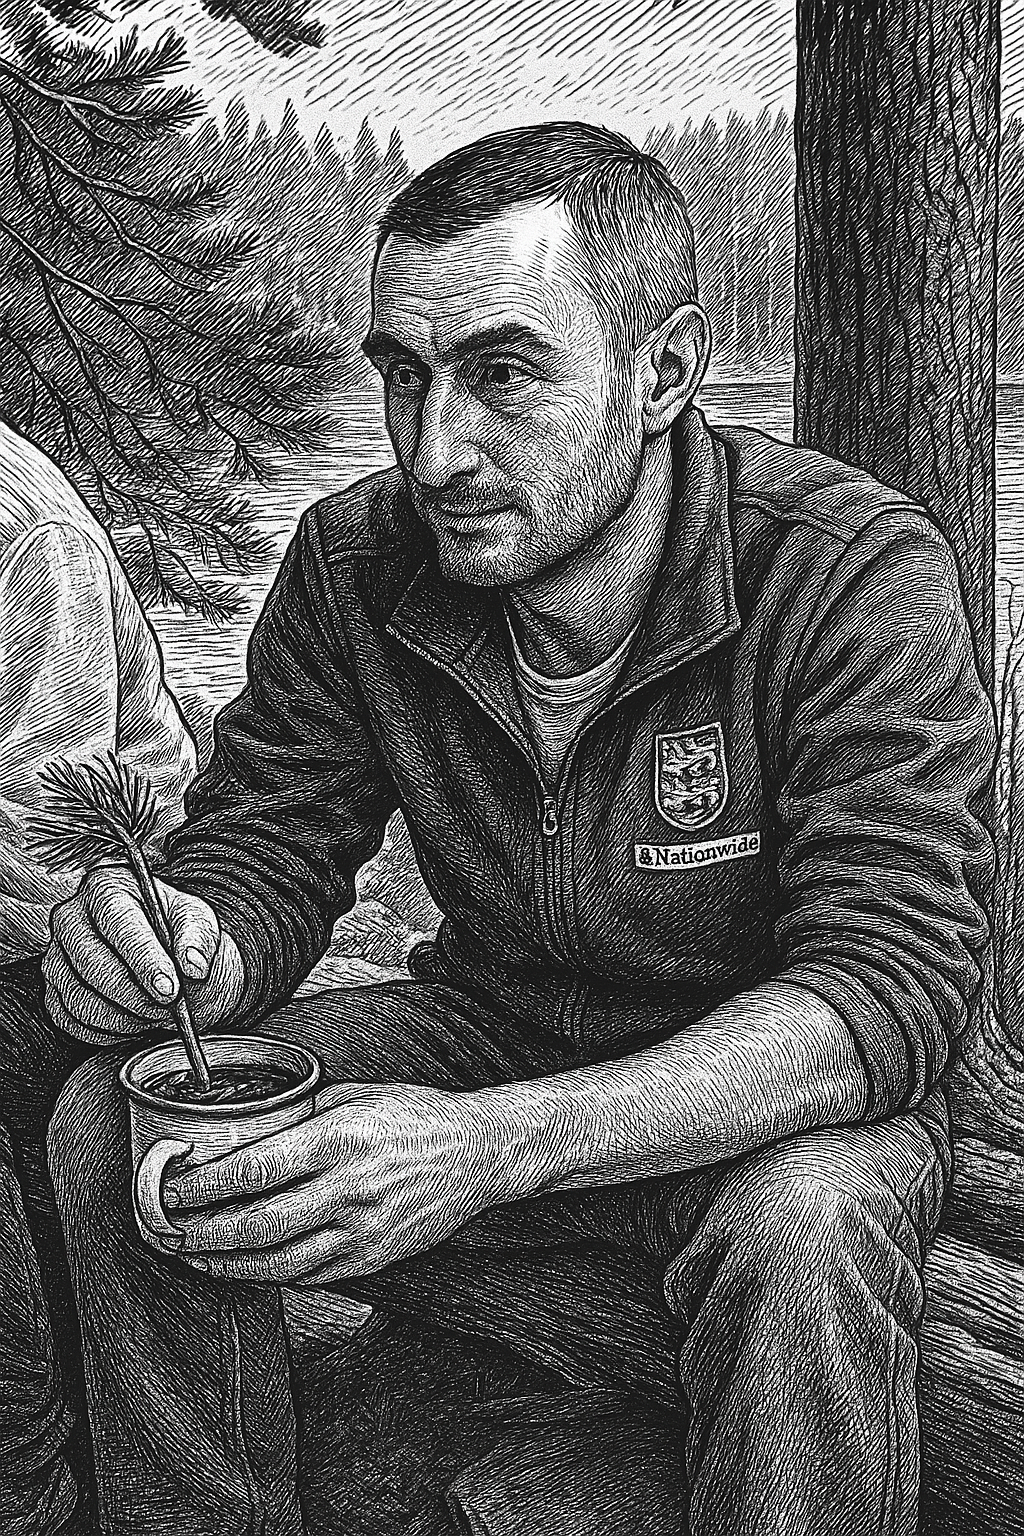
\includegraphics[width=0.48\textwidth]{53_pasha}
	\caption{\small\textit{...Мешал чай...}}
	%\end{figure}
\end{wrapfigure}
\diagdash Ну вот. А на озере это чисто психологический эффект\mdash находишься в~отдалении от берега, плюс борта у байды низкие.

\diagdash Это да-а-а.\mdash согласился с Пашей Адмирал.

\diagdash Сколько нам до~конца ещё?\mdash подал голос Руслан.

Адмирал поперхнулся:

\diagdash Сплюнь, блин! До~антистапеля, не~конца! До~антистапеля осталось около десяти километров, что совсем уж немного.

\diagdash Суеверия, Шурик, суеверия!\mdash укоризненно покачал головой Серёга.

\diagdash Моряки ваще люди суеверные, знаешь ли. Суеверней только лётчики, и то не факт.

\diagdash Так мы, это, не моряки же.

\diagdash А кто?

\diagdash Речники!\mdash Замполит гордо встал и поднял кружку с~ромом.\mdash {\large SKÅ-Å-ÅL!!!}

\diagdash {\large SKÅ-Å-ÅL!!!}\mdash отозвалась команда, брякнув железными кружками.

\diagdash Я что\sdash то не заметил, как компотикопитие плавно перетекло в это.\mdash Адмирал закусил апельсином и затянулся сигарой$\ldots$

$\ldots$ На ужин Адмирал решил наварить борща:

\diagdash У~меня как раз осталось на~один раз заправку сделать. М? Кто\sdash нибудь против?

\diagdash Против борща? Шутишь?

\diagdash Чем помочь?\mdash предложил Руслан.

\diagdash Почисть остатки картофана, а~я~пока свеклой займусь. Овощной нож там в~кармане вещмешка.\mdash Адмирал нашёл последнюю свеклу и~лук с~морковкой.

\diagdash Шурик, ты нас балуешь!\mdash Серёга привалился к~сосне, сидя на бревне.

\diagdash Так я тоже ж кайфую\mdash и от приготовления всего этого, и от поглощения, так сказать. <<Фкусно жрать>>\mdash помнишь такое на ресурсе удава?

\diagdash Шурик, ты б ещё фидонет вспомнил, мамонт!

\diagdash Фидоху не застал, не надо меня в мамонты сразу!

Адмирал сделал зажарку, а потом наварил целый котелок борща. Парни принялись ужинать, времени было около восьми вечера. Паша как всегда организовал сальца, нарезав остатки. Замполит нарисовался на разлив:

\diagdash Сегодня ж последний вечер похода на реке, парни. Мы всегда когда раньше ходили в сплавы, в последний вечер подводили у костра итоги.\mdash поделился воспоминаниями с~командой Замполит.

\diagdash Это тема.\mdash поддержали все.

\begin{wrapfigure}[18]{l}{0.50\textwidth}
	%\begin{figure}[h]
	\centering
	\includegraphics[width=0.48\textwidth]{54_borsh}
	\caption{\small\textit{...Сделал зажарку...}}
	%\end{figure}
\end{wrapfigure}
\mdash Щас, пару строк ещё черкну в судовой журнал и приступим.\mdash Адмирал как раз дописывал страницу, пока Серёга разливал борщ.

Замполит начал:

\diagdash Ну, парни, спасибо, что все собрались в это путешествие! Потому что одной трепологии мало, надо взять и пойти, а это, знаете ли, не каждый сейчас в нашей действительности способен. % За нас! {\large SKÅ-Å-ÅL!!!}

\diagdash Поддерживаю,\mdash сказал Адмирал,\mdash далеко не каждый, увы! Я~с~трудом всегда наскребаю людей в сплав. Поэтому спасибо вам, парни, что доверились мне в который раз и пошли со~мной на пороги! И хотя не всё у нас было гладко, особенно на~Нурмисе и особенно с рациями,\mdash он красноречиво взглянул на Замполита,\mdash но мы всё преодолели\mdash и~пороги, и непогоду! Отдельно хочу отметить нашего Рыбака и~бесстрашного Вперёдсмотрящего$\ldots$

\diagdash Ой да харош, Сань!\mdash Пашка деланно засмущался.

\diagdash Не, не, всё правильно!\mdash Замполит стал считать улов:\mdash на уху на Мярандуксе наловил, щуку после порогов в Черанге вытащил, сегодня аж коптилку устроил!

\diagdash $\ldots$а также главного по компотам\mdash Серёгу, благодаря которому мы почти каждый день при витаминах,\mdash продолжил Адмирал.\mdash и при грибах, кстати! Лисички просто космос, Серёг. И на Мярандуксе тоже было зачётно! Отдельное спасибо Руслану за стойкость в перенесении погодных условий, и~в~целом по ситуациям. Поверь, для первого сплава\mdash у тебя всё прошло более чем круто! 

\diagdash Да, Шу-у-урик, тебе спасибо! Без тебя, конечно, никакого сплава бы не было, ты нас всех на это дело подбиваешь каждый раз.\mdash резюмировал Серёга.

\diagdash За Адмирала!\mdash поднял кружку Паша.

\diagdash За команду!\mdash поправил Адмирал.\mdash {\large SKÅ-Å-ÅL!!!}

\diagdash {\large SKÅ-Å-ÅL!!!}\mdash все отвалились в креслах, походных стульчиках или просто на брёвнах, закусив остатками апельсина.

Вокруг стало медленно темнеть, парни с удовольствием умяли борщ и продолжали посиделки, Замполит врубил свою колоночку, и Адмирал поставил музон. Колбаситься, как на Мярандуксе, никому уже не хотелось, они просто кайфовали от происходящего в целом, наслаждаясь природой и происходящим с ними.

\diagdash Возможно, это один из моих лучших походов.\mdash сказал Адмирал.

\diagdash Неплохой.\mdash отозвался Замполит.

\diagdash Ну-у-у, может потому что первый раз мы пороги взяли?\mdash предположили Серёга с Русланом.

\diagdash Да нет, не поэтому, пацаны,\mdash задумчиво протянул Адмирал,\mdash тут много факторов. Взять хотя бы погоду. Несмотря на~то, что для~похода в целом погода была как бы так себе и$\ldots$

\diagdash Шурик, не гневи богов, погода для Карелии была просто огонь! Это я тебе как человек всё детство проведший в Карелии говорю!

\diagdash $\ldots$на штурм порогов пошёл дождь, да и вообще, можно было и получше$\ldots$

\diagdash Шурик, для Карелии\mdash это было пять звёзд, реально.\mdash настаивал Замполит.

\diagdash Да? Ну ладно.\mdash нехотя сдался Адмирал.\mdash Я~не~то совсем сказать\sdash то хотел. Я говорю, он мне кажется одним из~лучших, потому что как\sdash то органично всё прошло, всё как надо. И без потерь.

\diagdash На душу легло, да?\mdash подытожил Серёга.

\diagdash Да-а-а.\mdash согласились все.

\diagdash Легло, не представляешь как!\mdash Адмирал закрыл глаза.\mdash Может потому что первый раз по маршруту, а~может ещё чего. По Чагодоще когда ходили\mdash тоже в~первый раз было ярко и мощно, а потом уже всё не то. По~Песи ярко мы тогда прошли$\ldots$

\diagdash Тогда это не от похода зависит как такового же, а от новых ощущений.\mdash сказал Паша.\mdash по Чагодоще потом уже когда ходили, ты расстраивался, что стоянки наши заняты, что всё не~повторяется точь\sdash в\sdash точь, как при прошлом прохождении. В~этом и~суть. А~в~этот раз у~нас первопроход маршрута, и просто не~на~что ориентироваться. Ну~кроме отчётов чужих, но~это~не~то~немного.

\diagdash Доля истины в этом есть.\mdash согласился Замполит.

\diagdash Пожалуй так.\mdash Адмирал копался в памяти.\mdash Но всё равно тянет повторить некоторые маршруты, хотя знаешь, что былого не вернуть.

\diagdash Такова жизнь.

\diagdash Увы!\mdash согласилась команда.

\diagdash Ладно, чего загрустили? Поход по кайфу прошли. Разливай, тащ Замполит! И врубите уже Цоя, ну$\quldots$ %?$\ldots$?$\ldots$

\vspace{1em}
$\ldots$Cолнце давно село за лесом над Суной. Парни долго блаженствовали у костра, болтая о походе, жизни и~всякой ерунде, проводя последний вечер на реке. Ближе к~полуночи ром закончился, у~едва тлеющего костра остались только Адмирал с~Замполитом. Они, сидя в креслах, молчали, каждый думал о чём\sdash то своём, личном, и~лишь взошедшая над озером Луна была немым свидетелем того, как рвались в~клочья души походников$\ldots$ %от осознания того, что завтра их отчуждение от цивилизации закончится,


\begin{center}
	\psvectorian[scale=0.4]{88} % Красивый вензелёк :)
\end{center}
